% !TEX root = ../patchEmbeddings_review.tex

\begin{figure}[t]
\centering
        % \includegraphics[width=0.4\textwidth,trim=0.25in 0.25in 0.68in 0.36in,clip]{./figs/SSBM_experiments.pdf} % 0.45
        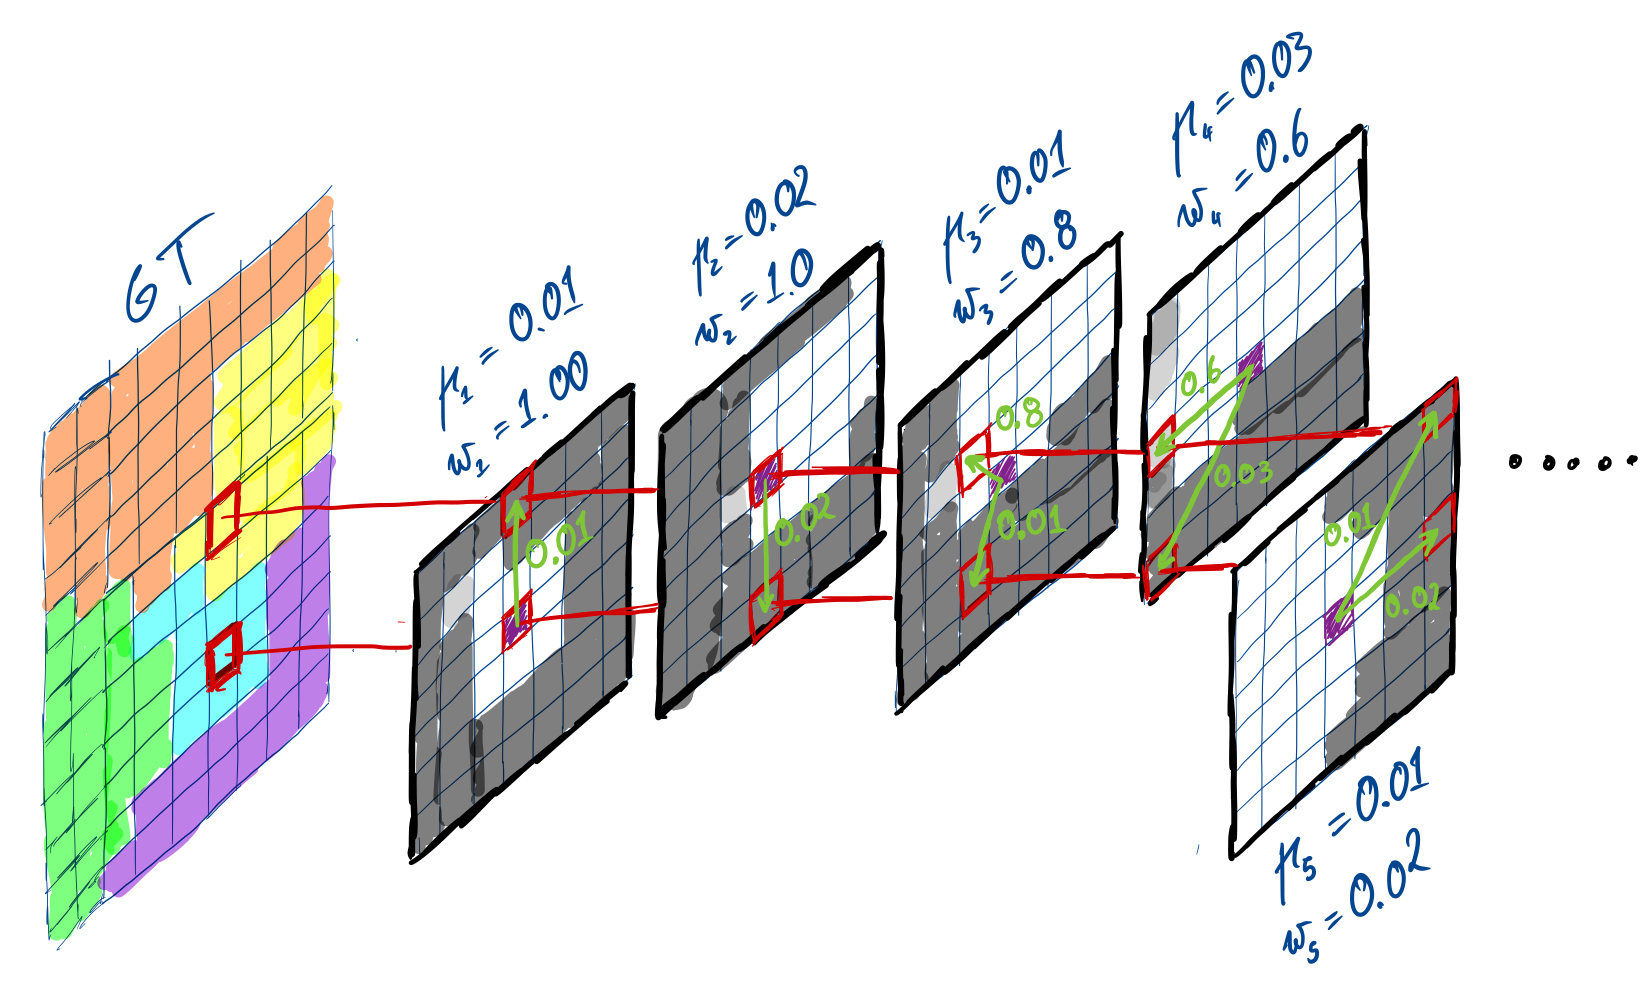
\includegraphics[width=0.7\textwidth]{./figs/alg_explaned.jpg} % 0.45
        \caption{Illustration of the proposed parameter-free method to convert \maskname masks to edge weights...}
    \label{fig:alg_explained}
\end{figure}
\begin{algorithm}[t]
  \begin{flushleft}
  \caption{: Affinities from aggregated \maskname masks}
   \hspace*{\algorithmicindent} \textbf{Input:} Graph $\mathcal{G}(V,E)$; \maskname masks $\mathcal{M}_{\coord{u}}: \mathcal{N}_{K\times K} \rightarrow [0,1]$  \\
  \hspace*{\algorithmicindent} \textbf{Output:} Affinities $\bar{a}_e\in[0,1]$ with variance $\sigma^2_e$ for all edges $e\in E$\\
  \hspace*{\algorithmicindent} 
  \begin{algorithmic}[1]
  \footnotesize
  % \small
      % \State Initial clustering: $\Pi=\{\{v_1\}, \ldots, \{v_{|V|}\}\}$
      % \State Initialize interactions between clusters with $ = w^+_e - w^-_e$
      \For{each edge $e\in E$ in graph $\mathcal{G}$}
        \State Get coordinates $\coord{u}=(u_x,u_y)$ and $\coord{v}=(v_x,v_y)$ of pixels linked by edge $e$

        % \State Init. accumulation sets $\mathcal{A}=\{\}$ for affinities and $\mathcal{W}=\{\}$ for reliability weights
        \For{each $i$-th mask $\mathcal{M}_{\coord{c}_i}$ including both pixel $\coord{u}$ and pixel $\coord{v}$}
            \State Get relative coords. of $\coord{u}$ and $\coord{v}$ with respect to the central pixel $\coord{c}_i$
            \State $a_i \gets \min \big(\mathcal{M}_{\coord{c}_i}(\coord{u} - \coord{c}_i), \,\mathcal{M}_{\coord{c}_i}(\coord{v} - \coord{c}_i)\big)$ \Comment{Fuzzy-AND: both values active}
            \State $\omega_i \gets \max \big(\mathcal{M}_{\coord{c}_i}(\coord{u} - \coord{c}_i), \,\mathcal{M}_{\coord{c}_i}(\coord{v} - \coord{c}_i)\big)$ \Comment{Fuzzy-OR: at least one value active}
        \EndFor
        \State Get weighted affinity average $\bar{a}_e= \sum_{i} a_i \omega_i\,/\,\sum_{i}\omega_i$ 
        \State Get weighted affinity variance $\sigma^2_e = \sum_{i} \omega_i (a_i-\bar{a}_e)^2\,/\,\sum_{i}\omega_i$
      \EndFor
      \State
      \Return $a_e, \sigma^2_e$ for each $e\in E$
  \end{algorithmic}
    \label{alg:computing_affinities}
  \end{flushleft}

\end{algorithm}

\section{Extracting affinities from \maskname masks}
In order to obtain an instance segmentation from the predictions of the model presented in Sec. \ref{sec:model}, we now compute instance-aware pixel-pair affinities for a given sparse $N$-neighborhood structure (see \TODO{Appendix} for details about the used structure) and use them as edge weights of a pixel grid-graph $\mathcal{G}(V,E)$, such that each node represents a pixel / voxel of the image. The graph is then partitioned to obtain object instances.
% \TODO{Section intro} Second contribution; two ways
% In this section, we propose two ways to perform something similar and use the predicted per-pixel \maskname masks to define the edge weights of a grid-graph.



\subsection{Efficient affinities for any sparse neighborhood}\label{sec:efficient_affs}
If the model is trained only with the \emph{\sparseBr branch} shown in Fig. \ref{fig:main_figure}a, then the desired $N$-neighborhood structure defining the connectivity of the grid-graph has to be defined before training. 
On the other hand, if the model is trained with the \emph{\encBr branch} of Fig. \ref{fig:main_figure}c, then the sparse connectivity structure of the graph can be defined at prediction time, but the \emph{\maskDec} network of Fig. \ref{fig:main_figure}c has to be applied to each pixel of the image in order to predict the desired affinity values, given by the value of $N$ in each mask. 
Alternatively, another much more efficient method consists in predicting these affinities directly from the $Q$-dimensional latent space of the encoded masks, by stacking few additional convolutional layers that do not need to be jointly trained with the full model and only serve to convert the encoded latent space to the desired $N$ output feature maps.
% ,  predict  from the previously trained latent space feature maps $Q\times H\times W$.
In this way, the graph $N$-neighborhood structure can be defined at prediction time, but the resulting model is no more memory-consuming than one directly trained to predict only that specific neighborhood. 



\subsection{Affinities with uncertainty from aggregated masks}\label{sec:aggr_affs}
As an alternative to the efficient method proposed in Sec. \ref{sec:efficient_affs}, in this section we propose an algorithm that, without the need of any threshold parameter, aggregates predictions from overlapping \maskname masks and output edge weights with associated uncertainty.

Related work either threshold the predicted \maskname masks \cite{januszewski2018high,hirsch2020patchperpix,meirovitch2016multi} or compute Intersection over Union (IoU) scores for overlapping patches \cite{liu2016multi}. However, an advantage of predicting pixel-pair affinities / pseudo-probabilities as compared to IoU scores is that affinities can easily be translated into attractive and repulsive interactions in the grid-graph 
% i.e. edge with either positive or negative weights, 
and a parameter-free partitioning algorithm can be employed to yield instances.
% Related work in \cite{liu2016multi} aggregate \maskname masks by computing Intersection over Union (IoU) scores for overlapping patches, however these scores cannot be translated into attractive and repulsive cues of the graph, so hierarchical agglomerative clusterings 

Here, we propose a simple method to aggregate predictions from multiple patches (see Algorithm \ref{alg:computing_affinities} and Fig. \ref{fig:alg_explained}). Let us assume we want to compute the weight for an edge $e$ linking pixels $\coord{u}$ and $\coord{v}$. Then we consider all predicted \maskname masks covering both $\coord{u}$ and $\coord{v}$. For example, if $\coord{u}$ and $\coord{v}$ are direct neighbors and the predicted masks have shape $K\times K$, then there will be $K(K-1)$ predicted masks including both pixel $\coord{u}$ and $\coord{v}.$\footnote{Note that here we ignore possible boundary effects by considering two pixels close to the image border.} 
For each considered mask $\mathcal{M}_{\coord{c}}$ centered at pixel $\coord{c}$, we consider three possible cases: i) both pixels are included in the $\coord{c}$ \maskname mask and by transitivity they should also be in the same instance and have high affinity and tendency to be in the same cluster
In summary, if both of them (fuzzy AND operator $min()$) belong to the mask centered at $\coord{c}$, then there is evidence for them to belong to the same cluster (affinity $a_i$ close to one). 
From mask $\mathcal{M}_{\coord{c}_i}$, something can be said about the pairwise affinity between $\coord{u}$ and $\coord{v}$ only when at least one of them belong to the $\coord{c}$-\maskname mask (fuzzy OR operator $max()$). If both of them are out of the mask (Fig. \ref{fig:alg_explained}c), then there is no evidence at all from this mask (reliability weight $\omega_i$ close to zero).

\begin{itemize}
\item Implemented on GPU (and online algorithm for variance)
\item variance interpreted as ``how consistent were the predictions of the masks for this particular edge weight''

\end{itemize}




